\documentclass[a4paper,12pt,titlepage]{extarticle}
%\usepackage{usu8}
\usepackage[utf8]{inputenc}
\usepackage[english,russian]{babel}
\usepackage{graphicx}
\usepackage{amssymb}
\usepackage{amsmath}
\usepackage[left=20mm,right=15mm,top=20mm,bottom=20mm,bindingoffset=0cm]{geometry}
%left 20..30, right 10..15
\renewcommand{\baselinestretch}{1.5} % 1.5 .. 2.0
%font height >=1.8, 2.5 .. 2.7
\usepackage{tocloft}
\renewcommand{\cftsecleader}{\cftdotfill{\cftdotsep}}

\def \title {О способах и технологиях расширения языков программирования}
\def \author {Мелентьев Артем Алексеевич}
\def \date {Екатеринбург -- 2009}
\def \supergrade {ассистент кафедры алгебры и дискретной математики, к.ф.-м.н.}
\def \super {Клепинин Александр Владимирович}
\def \spec {Специальность 010109 --- <<Дискретная математика и математическая кибернетика>>}
\def \grade {Диссертация на соискание академической степени магистра физико-математических наук}

\begin{document}
\begin{titlepage}\begin{center}
\normalsize
Федеральное агентство по образованию РФ \\
Государственное образовательное учреждение высшего профессионального образования \\
Уральский государственный университет им. А.М.Горького \\
\vfil
Математико-механический факультет \\
Кафедра алгебры и дискретной математики \\ 
%\hrule 
\vfil
\large \author\\
\LARGE \title\\
\small \spec\\
\small \grade\\
\vfil
\begin{flushright}
\begin{minipage}[]{250pt}
%\begin{center}
\normalsize научный руководитель:\\
\normalsize \supergrade\\
\normalsize \super\\
%\end{center}
\end{minipage}
\end{flushright}
\vfil
\normalsize \date
\vfilneg
\end{center}\end{titlepage}

\renewcommand{\abstractname}{Реферат}
\begin{abstract}
Мелентьев А.А. ``О способах и технологиях расширения языков программирования'',
квалификационная работа на степень магистра наук: стр.39, рис.4, библ.19.
назв. \newline \newline
Ключевые слова: расширяемый язык программирования, расширение языка, синтаксис,
создание расширений.
\newline \newline
В работе произведено сравнение и классификация различных средств для расширения
как синтаксических, так и семантических возможностей некоторых языков
программирования. Также приведены способы создания таких средств.
\end{abstract}

\setcounter{page}{3}
\renewcommand{\contentsname}{Оглавление}
\tableofcontents

\pagebreak

\section{Введение}

В процессе разработки ПО, как правило, используются универсальные языки
программирования, возможностей которых зачастую не хватает для многих областей.
Естественным образом появляется задача подгонки возможностей языка под
конкретную предметную область. Отсюда возникает задача исследования как общих
подходов к расширению языков, так и расширений конкретных языков
программирования.

История расширяемых языков программирования начинается в 60-ых годах с работ о
макросах и компиляторах компиляторов. Область активно развивалась и конечной
целью было создание действительно расширяемого языка программирования. В
то время был представлен проект расширяемого языка программирования Simula. Но
его расширяемость воплотить так и не удалось из-за возникших сложностей.
Интерес к области стал снижаться в 70-ых годах. Одним из объяснений
этого является чрезмерная сложность создания расширений. Активный интерес к
области вновь появляется в начале 21 века. Из за всеобщей компьютеризации
многим областям стали необходимы специальные языки программирования, а развитие
методов программирования позволило создавать сложные расширяемые языки.
Подробней про историю расширяемых языков можно прочитать в разделе \ref{hist}.

В настоящее время область расширяемых языков очень большая и активно
развивающаяся, но она мало структурирована. Существует множество расширений
различных языков. Некоторые из них заброшены, а некоторые до сих пор успешно
используются. Существует несколько компиляторов, которые заявляют о своей
расширяемости. Естественным образом возникает вопрос: какой из них более
расширяем и требует минимум знаний и усилий для расширения? Также существует
огромное количество инструментов для создания компиляторов. И также возникает
вопрос: какие из них лучше подходят для создания именно расширяемых
компиляторов или для одиночных расширений языка? В данной работе сделана
попытка обзора, классификации и структуризации различных технологий, проектов,
способов используемых в расширяемых языках и в одиночных расширениях языков.
Также построен возможный план создания идеального расширяемого компилятора.

TODO: повтор?
Перед автором была поставлена задача: исследовать наработки в области 
расширений языков а также классифицировать и структурировать их.
Задача была успешно выполнена, а именно в работе привен обзор исследованых
расширений, сделана попытка их классификации и структуризации по общим
признакам. Более того, приведен возможный план создания расширяемого
компилятора на основе изученных технологий.

По-настоящему расширяемые языки даже в настоящее время очень трудно
реализуемы. Помимо обеспечения расширяемости, трудности возникают с
совместностью расширений и их отладкой. Также некоторые опасаются, что
расширяемые языки затруднят взаимодействие программистов, так как будут
поощрять создание индивидуальных расширений ``под себя'', что каждый будет
писать на своем диалекте языка, несовместимом с диалектом другого.

Существуют проекты, как например SQLj \cite{sqlj}, которые являются одиночными
расширениями базового языка и не позволяющие дальнейших расширений (по
крайней мере внешне). Такие расширения в работе также исследуются.

В развивающихся языках тоже можно проследить расширения. Так, например, в язык
C\# в каждой версии добавляется множество синтаксических расширений. Наиболее
значительные из них появились в версии 3.0. Но их сложно оценивать с точки
зрения создания расширений, так как это внутренние расширения, сильно связанные
с языком. В большинстве языков программирования нет системы создания
расширений, и для их создания требуется глубокое знание устройства компилятора.

В отличие от C\#, язык Java более консервативней в развитии и синтаксически
меньше. Java специально создавался синтаксически минимальным для облегчения
взаимодействия программистов. Отчасти, благодаря этому Java сейчас
является наиболее популярным языком программирования \cite{tiobe}. Вследствие 
большого сообщества и большей необходимости расширений, у языка Java
гораздо больше внешних расширений и исследований в этой области чем у C\#.
Поэтому в данной работе в основном исследуются расширения языка Java и смежных
языков. Автор также не скрывает большого опыта работы с ним и личного
предпочтения.

Для создания расширений с нуля используется множество инструментов, облегчающих
их создание: генераторы лексеров, генераторы парсеров, компиляторы
компиляторов, различные вспомогательные библиотеки, средства связи со средой
разработки и прочее. Все это будет рассмотрено в главе \ref{tools}.

Работа устроена следующим образом. Во введении далее идет обзор типичной
структуры компилятора и его возможных точек расширения и список определений,
используемых в работе. За ним идет исторический обзор области и её текущее
состояние. В главе \ref{clas} произведена попытка обзора и классификации текущих
проектов области. И в главе \ref{tools} содержится обзор инструментов для
создания расширений языков. Почти все приведенные в работе программные проекты
доступны в исходных кодах. Закрытых проектов в данной области очень мало.

\subsection{Точки расширения компилятора}
Для того, чтобы расширить компилятор, сначала необходимо понять его структуру.
Рассмотрим примерную структуру компилятора:
\begin{center}
 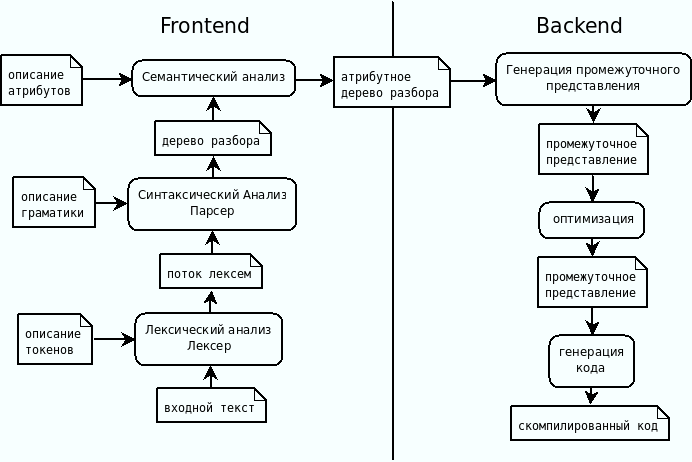
\includegraphics[scale=0.6]{img/compiler2.png}
\end{center}
Здесь листки обозначают данные, а закругленные прямоугольники - процессы.
\newline \newline
Процесс компиляции обычно состоит из следующих этапов:

\begin{enumerate}
  \item Лексический анализ. Лексер. На этом этапе последовательность символов
  исходного файла преобразуется в последовательность лексем, то есть пар (идентификатор
  лексемы, последовательность символов). Лексемы также часто называют токенами.
  Модуль, отвечающий за лексический анализ, называется лексером или
  токенайзером. Не все компиляторы имеют выделенный лексический анализатор,
  поскольку он может являться незаметной частью синтаксического анализатора.
  \item Синтаксический (грамматический) анализ. Парсер. Последовательность
  лексем преобразуется в дерево разбора в соответствии с грамматикой языка.
  Модуль, отвечающий за синтаксический анализ, называется парсер. Дерево
  разбора тут понимается в общем смысле. Обычно в синтаксическом анализе
  используется синтаксическое дерево (Abstract Syntax Tree, AST), которое
  отличается от дерева разбора отсутствием несущественных грамматических элементов
  (например: запятые, скобки, ключевые слова. их можно восстановить по
  типу и структуре узлов AST).
  \item Семантический анализ. Дерево разбора обрабатывается с целью
  установления его семантики (смысла). Например, привязка идентификаторов к
  их декларациям, типам, проверка совместимости, определение типов выражений и
  т.д. Результатом обычно является расширенное дерево разбора. Часто
  семантический анализ делается с помощью атрибутной грамматики, и в результате
  получается расширенное атрибутами дерево разбора.
  \item Генерация промежуточного представления. По данным семантического
  анализа создается удобное представление для дальнейшей оптимизации и
  генерации кода, например, в форме какого нибудь специального высокоуровнего
  ассемблера.
  \item Оптимизация. Выполняется удаление излишних конструкций и упрощение кода
  с сохранением его смысла. Оптимизация может производиться на разных уровнях и
  этапах: например, над промежуточным кодом или над конечным машинным кодом.
  \item Генерация кода. Из промежуточного представления порождается код на
  целевом (обычно машинном) языке.
\end{enumerate}
В конкретных реализациях компиляторов эти этапы могут быть разделены или
совмещены в том или ином виде.

Три первых этапа (также, возможно, с включением последующей генерации
промежуточного представления) часто называют фронтендом (frontend) компилятора.
А 3 последних этапа -- бэкендом (backend). Фронтенд и бэкенд --- это общие
понятия, обозначающее соответственно начало и конец процесса. Причем возможно
наличие нескольких взаимозаменяемых фронтендов и бэкендов. Например, в
известном наборе компиляторов Gnu Compiller Collections фронтендами являются
распознаватели языков программирования C, C++, Pascal, Java, Ada и др. А
бэкендами -- оптимизаторы и генераторы кода под соответствующую архитектуру процессора
(x86, arm, mips, и др.) и операционную систему)

Итак, что же можно расширить в данной схеме? Почти все, если иметь доступ к
соответствующим частям компилятора. Традиционные компиляторы этот доступ вовне
не предоставляют. И даже если бы и предоставили, то в больших компиляторах он
был бы чрезвычайно сложен.. Поэтому в большинстве случаев внешние расширения
создают путем внедрения в начало этой схемы своего препроцессора или генератора
кода из своего языка на на исходный язык компилятора.

Но, допустим, у нас есть удобный доступ ко всем структурам компилятора. Тогда
появляются следующие возможности:

\begin{enumerate}
  \item Лексер. Расширением лексера можно ввести новые лексемы, которые могут
  быть затем использованы в синтаксическом анализаторе. Также можно сменить
  оформление программы, например в компиляторе Nemerle опциональным расширением
  лексера достигается поведение отступов как в Python (``лесенка'' задает
  структуру программы, т.е. расставляет блоки фигурных скобок).
  \item Парсер. Наиболее интересное место для расширений. Здесь можно добавить
  новые синтаксические конструкции или изменить старые.
  \item Семантический анализатор. Тут добавляется семантика новым
  синтаксическим конструкциям. Можно, например, свести новые конструкции к
  старым, чтобы не заниматься генерацией их промежуточного представления.
  Также можно добавить какую-нибудь новую семантику существующим
  синтаксическим конструкциям.
  \item Бэкенд. Тут возможны дополнительные оптимизационные проходы, генерация
  дополнительного (например, отладочного) кода.
\end{enumerate}
Проблема тут в том, что почти любая такая модификация компилятора требует его
пересборки. Например малейшее изменение грамматики требует полной пересборки
парсера. Таким образом, пользовательские расширения компилятора сильно
затруднены. Но расширяемые компиляторы, про которые будет написано в разделе
\ref{extcomp}, пытаются преодолеть эти проблемы различными способами.

\subsection{Определения}

Приведем некоторые определения, используемые в области:
\begin{enumerate}
  \item Язык предметной области (Domain Specific Language, DSL) --- это
  специально разработанный язык для решения определённого круга задач, в
  отличие от языков программирования общего назначения. Как правило
  сильно повышает продуктивность работы в этой области, в отличие от
  универсальных языков. Существуют внутренние и внешние DSL.
  \item Внутренний DSL (embedded или internal DSL) --- это DSL внутри другого
  языка. В языке создается своего рода мини язык через синтаксические
  возможности базового языка. Таким образом, программа на внутреннем DSL
  является и программой на базовом языке. В языках семейства Lisp внутренние
  DSL наиболее легко реализуемы.
  \item Внешний DSL --- это DSL не связанный с базовым языком, в отличие от
  внутреннего DSL. Он требует отдельного парсера для распознавания. В качестве
  примера можно привести файлы описания сборки (makefile)
  \item Языково-ориентированное программирование (ЯОП, Language oriented
  programming, LOP) --- стиль программирования, в котором в отличие от решения
  задач на универсальных языках, программист сначала создает один или несколько
  DSL для задачи, и потом решает задачу на этих языках. Понятие ЯОП пришло из
  языка Lisp, где из-за синтаксических возможностей широко практикуется
  создание внутренних DSL. Про языки семейства Lisp подробнее написано в
  разделе \ref{lisp}.
\end{enumerate}

\section{Обзор области}

\subsection{История}
\label{hist}
Область расширяемых языков программирования впервые появилась в 60-ых годах
\cite{hist69}. Первая научная работа -- ``Макросы для высокоуровневых языков
программирования'' принадлежит Дугласу Маклрою (M. Douglas Mcllroy's)
\cite{macro60}. Другие ранние описания принципа расширяемости приводятся в
статье Брукера и Мориса про компилятор компиляторов \cite{cc60}.
Пик движения отмечен двумя академическими симпозиумами в 1969 \cite{proc69} и 1971
\cite{proc71}. Обзорная статья по данной области была написана в 1975 году
Томасом Стандишом \cite{Stan75}, после чего интерес к области начал пропадать.
Но интерес к области вновь резко возрастает в 21-ом веке \cite{Ext2105}.

\subsubsection*{Характеристика ранних подходов}

Расширяемый язык программирования состоит из простого базового языка и
метаязыка, способного изменять базовый язык. Расширенный язык получается
модификациями базового языка с помощью метаязыка. Большинство техник расширений
языка в то время были макроподстановками. Тем не менее модификации грамматик 
также исследовались, и в результате появились адаптивные грамматики, способные
изменять свой синтаксис прямо во время выполнения. Про них подробнее будет 
рассказано в разделе \ref{adaptive}. Сообщество языка Lisp оставалось отделенным
от сообщества исследователей расширяемых языков, видимо потому что, как один
исследователь заметил в \cite{harr60}:
\begin{quote}
``любой язык программирования, в котором программа и данные существенно
неразличимы, может считаться расширяемым языком. \ldots это легко можно увидеть
из того факта, что Lisp использовался как расширяемый язык многие годы''
\end{quote}
На конференции 1969 года был представлен Simula как расширяемый язык
программирования, но в силу возникших трудностей его расширяемость так и не
была реализована.

Стандиш описал три класса расширений языка, которые он назвал перефраз
(paraphrase), ортофраз (orthophrase) и метафраз (metaphrase).
\begin{itemize}
  \item Перефраз добавляет новые возможности, сводя их к уже имеющемуся. В
  качестве примера можно привести макроподстановки, которые в конечном счете
  разворачиваются в конструкции базового языка.
  \item Ортофраз добавляет возможности, невыразимые в базовом языке, такие как,
  например, добавление системы ввода-вывода к языку, не имеющему оной. Таким
  образом, ортофраз-расширение должно быть написано на другом языке. Из
  современных понятий близким аналогом является понятие подключаемого дополнения
  (plug-in).
  \item Метафраз модифицирует интерпретацию существующих элементов языка, и,
  таким образом, выражения разбираются по-новому. Оно соответствует
  современному понятию рефлексии.
\end{itemize}

\subsubsection*{Закат ранних подходов}

Стандиш аргументировал неудачу движения сложностью программирования последующих
расширений. Обычный программист может создать некое расширение вокруг базового
языка, но если второе расширение будет создано вокруг первого, то программисту
нужно быть близко знакомым и с базовым языком, и с первым расширением. Третье
расширение будет требовать еще больше знаний и так далее. Следует заметить, что
отделение программиста от низкоуровневых деталей -- это цель области
абстракции, которое вытеснило область расширяемости в то время.

\subsection{Современное состояние}
\label{modernextsys}

В современном смысле система, поддерживающая расширяемое программирование,
предоставляет все нижеперечисленные возможности:

\subsubsection*{Расширяемый синтаксис}

Это просто означает, что язык не должен быть фиксированным или статичным. Он
должен предоставлять возможность добавлять новые синтаксические конструкции.
Допустима неизменность некоторых фундаментальных и внутренних свойств языка, но
система не должна полностью от них зависеть.

\subsubsection*{Расширяемый компилятор}

В расширяемом программировании компилятор не является монолитной программой,
которая преобразует исходный код в бинарный исполняемый формат. Компилятор сам
должен быть расширяем через набор дополнений, которые помогают в преобразовании
исходного языка во что угодно. Например, расширяемый компилятор будет
генерировать объектный код, документацию к коду, переформатированный исходный
код или любую другую желаемую информацию. Архитектура компилятора должна
предоставлять интерфейсы для доступа внутрь процесса компиляции и предоставлять
возможность использовать альтернативные задачи обработки на каждый разумный шаг
процесса компиляции.

Для простой задачи трансляции исходного кода в что-либо, способное запуститься
на компьютере, расширяемый компилятор должен:

\begin{itemize}
  \item Использовать модульную (plug-in) или компонентную архитектуру для почти
  каждого шага компиляции.
  \item Определить язык или вариант языка, который будет компилироваться, и
  найти подходящий компонент для распознавания и проверки этого языка.
  \item Проверять семантическую правильность путем запуска соответствующего
  компонента.
  \item Иметь возможность выбора из нескольких генераторов кода для разных
  процессоров, операционных систем, виртуальных машин и пр.
  \item Предоставить методы для генерации ошибок и их расширения.
  \item Предоставить возможность добавлять новые узлы, значения и ребра в
  синтаксическое дерево.
  \item Предоставить возможность трансляции и трансформации синтаксического
  дерева или поддерева через внешние компоненты.
  \item Обеспечить поток информации между внутренними и внешними компонентами
\end{itemize}

\subsubsection*{Расширяемая среда исполнения}
Среда исполнения расширяемой системы программирования должна позволять языкам
расширять множество допустимых операций. Например, если система использует
интерпретатор байт-кода, то она должна иметь возможность определения новых
команд и соответствующих им представлений в байт-коде. Как и в расширяемом
синтаксисе допустимо наличие небольшого набора неизменных фундаментальных
внутренних инструкций. Тем не менее, должно быть возможно перегрузить
(overload) эти операторы так, чтобы появились новые или дополнительные
возможности.

\subsubsection*{Отделение содержания от формы}
Расширяемые системы программирования должны рассматривать программы как данные
для обработки. Эти программы должны быть полностью лишены любой информации о
форматировании. Система должна преобразовать программу в форму, наиболее
подходящую для просмотра, редактирования или генерации кода.

\subsubsection*{Поддержка отладки создаваемых языков}
Расширяемая система программирования должна поддерживать отладку программ,
используя конструкции языка, на котором она записана, вне зависимости от
количества расширений языка и трансформаций программы. Отладчик должен
позволять отображать данные в форме, подходящей для языка. Например, если язык
поддерживает структуры данных для бизнес процессов или потоков выполнения, то
его отладчик должен выводить эти структуры в виде диаграмм Ишикавы
\cite{ishikawa} (Ishikawa, fishbone, cause-and-effect diagrams) или в другой
форме, предоставляемой неким специальным компонентом.

Такое современное определение расширяемой системы программирования требует
очень многого. Получился своего рода идеал. Истинно расширяемых систем в таком
понимании на данный момент нет. Наиболее близким к данному определению
является, наверное XLR: Extensible Language and Runtime, про который подробнее
написано в \ref{xlr}. В данной работе расширения будут рассматриваться в более
общем смысле.

\section{Классификация}
\label{clas}

Расширения компилятора можно условно подразделить на синтаксические и
семантические. Синтаксические расширения добавляют новые синтаксические
конструкции в язык. Пример -- перечисления (enum), обобщенные типы (generics) в
Java~5. Семантические расширения, в отличие от синтаксических, просто меняют
поведение кода без введения новых синтаксических конструкций. Примером
семантических расширений является аспектно-ориентированное программирование
(АОП), которое будет рассмотрено в разделе \ref{aop}.

\subsection{Семантические расширения}

Семантические расширения меняют поведение программы каким-либо внешним образом.
Например через препроцессор исходного или байт-кода.
Рассмотрим представителей данного класса:

\subsubsection*{Метапрограммирование}
Метапрограммирование — область ориентированная на создание программ, которые
создают другие программы как результат своей работы (либо, в частном случае,
изменяющие или дополняющие себя во время выполнения).

Метапрограммирование разделяется на 2 направления: на стадии
компиляции (генерация кода) и на стадии выполнения (самомодифицирующийся код).

Первое направление позволяет получить программу при меньших затратах времени и
усилий, чем если бы программист писал её вручную. Второе — расширяет
возможности программиста.

\subsubsection*{Аспектно-ориентированное программирование}
\label{aop}
Аспектно-ориентированное программирование (АОП) — это методика программирования
в рамках классовой парадигмы, основывающая на понятии аспекта — блока кода,
инкапсулирующего сквозное поведение в составе классов и повторно используемых
модулей.

Аспектно-ориентированное программирование выросло из осознания того, что в
типовых программах на объектно-ориентированных языках часто представлено
поведение, которое не вмещается естественно в один или даже в несколько тесно
связанных программных модулей. Пионеры аспектного подхода ввели термин
«пересечение» (crosscutting, сквозная функциональность) для обозначения
поведения кода, при котором пересекаются ответственности разработчиков
программных модулей. В объектно-ориентированном программировании, например,
единицей модульности является класс, а «секущее» свойство охватывает несколько
классов. Часто пересечение встречается при организации журналирования
приложений, контекстно зависимой обработке ошибок, оптимизации выполнения
программ, а также в шаблонах проектирования.

АОП дополняет объектно-ориентированное программирование, обогащая его другим
типом модульности, который позволяет локализовать код реализации crosscutting
логики в одном модуле. Такие модули обозначаются термином аспекты, от
аспектно-ориентированного программирования. За счет отделения
аспектно-ориентированного кода работа с crosscutting-отношениями упрощается.
Аспекты в системе могут изменяться, вставляться, удаляться на этапе компиляции
и, более того, повторно использоваться.

Все языки АОП предоставляют способы для выделения сквозной функциональности в
отдельную сущность. Различие между ними заключается в удобстве, безопасности и
области применения средств, которые они предоставляют. Наиболее популярный на
данный момент язык АОП — AspectJ. Используемые в нем понятия распространились
на большинство языков АОП.

Рассмотрим AspectJ на примере аспекта для журналирования событий. Допустим у
нас есть множество методов doSomething, в которых необходимо журналировать
моменты входа и выхода, например:
\begin{verbatim}
public void doGet(JspImplicitObjects theObjects) throws ServletException 
{
  logger.entry("doGet(...)");
  JspTestController controller = new JspTestController();
  controller.handleRequest(theObjects);
  logger.exit("doGet");
}
\end{verbatim}
Вручную писать журналирование для каждого метода требует существенных усилий, и
может привести к трудно выявляемым ошибкам, если программист немного ошибется
в строке журналирования. Это задача легко решается введением сквозной
функциональности через следующий аспект:
\begin{verbatim}
public aspect AutoLog 
{
  pointcut publicMethods() : execution(public * my.package..*(..));
  pointcut logObjectCalls() : execution(* Logger.*(..));
  pointcut loggableCalls() : publicMethods() && ! logObjectCalls();
  before() : loggableCalls() {
    Logger.entry(thisJoinPoint.getSignature().toString());
  }
  after() : loggableCalls() {
    Logger.exit(thisJoinPoint.getSignature().toString());
  }
}
\end{verbatim}
Проанализируем этот пример и посмотрим, какие действия осуществляет аспект.
Первое, на что нужно обратить внимание — это объявление аспекта. Оно подобно
объявлению класса и, так же как класс, определяет тип Java. Кроме того, аспект
содержит конструкции pointcut и advice.

Прежде всего, рассмотрим, что представляет собой join point (точка соединения).
Точки соединения --- это однозначно определенные точки при выполнении программы.
Так под точками соединения в AspectJ подразумеваются: вызовы методов, точки
обращения к членам класса и исполнение блоков обработчиков исключений и т. д.
Точки соединения могут, в свою очередь, содержать другие точки соединения.
Например, результат вызова метода может передаваться каким-то другим методам. А
pointcut является языковой конструкцией, которая отбирает множество точек
соединения на основании определенного критерия. В приведенном выше примере
первый pointcut под именем publicMethods выбирает исполнения всех public
методов в пакете my.package. Подобно int, который является базовым типом
Java, Execution является базовым pointcut. Он выбирает исполнения методов,
соответствующих сигнатуре, заданной в скобках. Для сигнатур допустимо включение
символов шаблонов: в приведенном примере оба pointcut-а содержат несколько
таких символов. Второй pointcut с именем logObjectCalls выбирает все исполнения
методов в классе Logger. Третий pointcut loggableCalls, объединяет два
предыдущих, используя булевы операции \&\& и !, что означает выбор всех public
методов из my.package за исключением таковых в классе Logger. (Регистрация
методов в классе Logger привела бы в результате к бесконечной рекурсии).

Теперь, после того, как в аспекте определены точки, нужно использовать
конструкцию advice, чтобы выполнить текущую регистрацию. Advice — это фрагмент
кода, выполняющийся до, после или в составе точки соединения. Advice
определяется для pointcut, что представляет собой нечто наподобие указания
«выполнить этот код после каждого вызова метода, который надо регистрировать».
В итоге «След» вызова метода (с применением аспекта) в log-файле выглядит
примерно следующим образом:
\begin{verbatim}
Entering method: void test.Logging.main(String[])
Entering method: void test.Logging.foo()
exiting method: void test.Logging.foo()
exiting method: void test.Logging.main(String[]) 
\end{verbatim}

Pointcuts и advice позволяют влиять на динамику выполнения программы,
introduction предоставляет аспектам возможность модифицировать статическую
структуру программы. Используя introduction, аспекты могут добавлять новые
методы и переменные в классы, объявлять класс как реализацию интерфейса,
устанавливать или отменять проверку исключений.

У AspectJ существует хорошая инструментальная поддержка: среры программирования
Eclipse, NetBeans и Idea имеют расширения для удобной работы с AspectJ. AspectJ
легко применять и в системах сборки ant, maven.

Также интересно мнение стороников языка Лисп о AspectJ:
\begin{quote}
``В Лиспе, если охота аспектно-ориентированного программирования, нужно лишь
настругать немного макросов, и готово. В Java, нужен Грегор Кичалес, создающий
новую фирму, и месяцы и годы попыток заставить всё работать.'' (Петер Норвиг)
\end{quote}

АОП можно рассматривать как вариант метапрограммирования при компиляции.
Обычно аспекты описываются расширенным базовым языком, поэтому такое АОП можно
рассматривать и как синтаксическое расширение. Но существуют и реализации АОП
обходящиеся только средствами языка (например с помощью аннотаций Java~5).

\subsubsection*{Макросы}
 Макрос (от англ. macros, мн.ч. от macro) — программный объект, при обработке
«развертывающийся» в последовательность действий или команд. Таким образом
макросы можно отнести к метапрограммированию на стадии компиляции.

Макросы по отношению к языку можно разделить на внешние и внутренние.
Внешние макросы не связаны с языком, и не имеют доступа к контексту применения.
Пример внешних макросов -- препроцессор языка C, который реализован внешней
утилитой (cpp, The C PreProcessor) и никак не связан с языком.

Внутренние макросы, в отличие внешних, имеют доступ к контексту применения, и
поэтому обладают гораздо большей выразительной способностью. Как следствие,
внутренние макросы тесно связаны с языком. При применении они имеют доступ к
дереву разбора и могут изменять его.

Наиболее мощными внутренними макросами обладают языки семейства Lisp
(Common Lisp, Scheme). Языки Nemerle и Boo также обладает мощной встроенной
системой макросов, с помощью которых можно даже добавлять новые синтаксические
конструкции в язык. Для языка Java существует система внутренних макросов Java
Syntactic Extender, которая будет рассмотрена в разделе \ref{jse}.

\subsubsection*{Системы трансформации программ}
Техники трансформации программ используются во многих сферах: от генерации
программ, оптимизации и рефакторинга до обратной разработки и генерации
документации.
Данная область является, наверное, самой старой. Многие теории, инструменты и
приложения в этой области разработаны более 30 лет назад.
В связи большим возрастом области в ней сформировались некоторые стандарты.
В первую очередь это SDF \cite{sdf} -- syntax definition formalism, формат
файлов для описания грамматик контекстно-свободных языков. Форматом SDF пользуются
большинство систем трансформации.

Кроме того проект SDF предоставляет стандартный генератор парсеров класса SGLR
(Scanerless Generalized Left-to-right Rightmost derivation parser). SGLR иногда
называют параллельным парсером. Это расширение LR парсера, для поддержки
недетерминированных и неоднозначных грамматик. Алгоритмическая сложность разбора
= $O(n^3)$. При отсутствии неопределенностей - $O(n)$. Стоит заметить, что
большинство парсеров, используемых в компиляторах имеют линейную сложность,
поэтому кубическая сложность SGLR выглядит плохо. Но SGLR ценен тем, что может
распознавать недетерминированные и неоднозначные грамматики. Его соперниками
здесь являются LL(*) (требует специальных указаний для разрешения конфликтов) и
адаптивные грамматики (очень сложны). Большой класс распознаваемых языков
позволяет SGLR распознавать сложные языки и создавать большие расширения языков.

Некоторые системы трансформации:
\begin{itemize}
  \item Stratego/XT --- это язык трансформации Stratego и набор инструментов 
  XT для постоения систем трансформации. Язык Stratego основан на парадигме
  стратегической перезаписи термов (strategic term rewriting). Для описания
  грамматики используется стандартный формат SDF. На основе Stratego/XT создан
  фронтенд JavaFront, распознающий язык Java.
  \item ASF+SDF Meta Environment --- это среда и набор инструментов для
  интерактивного анализа и трансфориаций. ASF+SDF компинирует описанный
  выше Syntax Definition Formalism и Algebraic Specification Formalism (ASF) а
  также некоторые другие технологии. ASF используется для перезаписи термов.
  В отличие от Stratego/XT отличается ориентацией на среду программирования
  (MetaStudio IDE), визуализацию процессов.
  \item TermWare --- это система обработки термов, предназначенная для
  встраивания в Java приложения. TermWare не использует SDF, и вообще не
  содержит своего парсера. Сам TermWare предназначен только для обработки
  термов. На основе TermWare и JavaCC создан фронтенд JavaChecker, распознающий
  язык Java и позволяющий проверять некоторые семантические ошибки используя
  правила TermWare. TermWare --- проект украинской фирмы gradsoft.ua.
\end{itemize}

\subsection{Синтаксические расширения}
Как уже было сказано, синтаксическое расширение добавляет в язык новые
синтаксические конструкции и связывает с ними какую-либо семантику.
Рассмотрим подробнее представителей этого класса.

\subsubsection*{Система Java Syntactic Extender}
\label{jse}
Java Syntactic Extender (JSE) --- расширение языка Java, позволяющее добавлять в
язык новые синтаксические конструкции. Оно основано на системе макросов Dylan с
учетом специфики языка Java. Расширения могут быть реализованы
непосредственно на Java без каких-либо ограничений. JSE - это
препроцессор языка Java, который разворачивает макросы.

JSE использует парсер языка Java с макросами, основанный на генераторе парсеров
ANTLR. Парсер строит специальное дерево разбора, оптимизированное для
макроподстановок, которое в JSE называется скелетное синтаксическое дерево
(Skeleton Syntax Tree, SST). В дальнейшем макросы явно или неявно манипулируют
именно SST.

Сами макросы представляют собой обычные классы Java, которые, имея доступ к
SST, разворачивают вызов макроса во что угодно. После применения всех макросов,
SST преобразуется обратно в текст для компиляции стандартным компилятором.

Недостатки:
\begin{itemize}
 \item не учитывается область видимости, возможен конфликт имен
 \item SST предоставляет мало контекстной информации
 \item проект заброшен. последняя версия 0.20 вышла в 2003 году.
\end{itemize}
Для успешности расширения языка нужна еще и его инструментальная поддержка.
Наиболее существенна поддержка среды программирования, которой у JSE небыло.
Наверное это и явилось причиной низкого интереса к этому проекту.

\subsubsection*{Язык OJ}
OJ -- бывшая OpenJava. Добавляет MetaObject Protocol в язык Java.
Позволяет изменять, создавать классы во время выполнения.
Проект заброшен. Возможно АОП оказалось более перспективным направлением.

\subsection{Расширяемые компиляторы}
\label{extcomp}
\subsubsection*{Компилятор Polyglot}
Polyglot - расширяемый текстовый преобразователь Java программ (транслятор из
Java в Java). Polyglot состоит из базового компилятора jlc и его расширений.
Компилятор jlc -- полноценный Java фронтенд. Он разбирает и проводит
семантический анализ исходного кода. Компилятор генерирует исходный Java код.
Таким образом, базовый компилятор не производит трансляции в байт-код, в
отличие от стандартного компилятора Java.

Языковые расширения реализуются поверх базового компилятора путем расширения
конкретного и абстрактного синтаксиса, системы типов и определения новых
трансформаций кода. В результате получается абстрактное синтаксическое дерево,
которое преобразуется в исходный код на Java и компилируется стандартным
компилятором javac.

\begin{center}
Фрагмент дерева языков, основанных на Polyglot:
\nopagebreak
 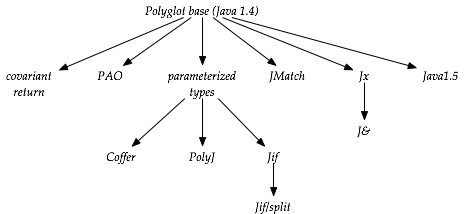
\includegraphics[scale=0.6]{img/polyglot-tree.png}
\end{center}

В Polyglot используется Polyglot Parser Generator~(PPG) -- собственный генератор
парсеров на основе JavaCUP \cite{javacup}.

Polyglot --- пример наиболее популярного подхода к созданию расширений языка:
сведение конструкций нового языка к конструкциям на базовом языке. Но, в
отличие от других подобных проектов, Polyglot смог собрать вокруг себя большое
сообщество, что привело к появлению многих расширений языка Java на его основе.
К сожалению, в последнее время активность проекта упала, и некоторые проекты
(например Soot, Aspect Bench Compiller(abc)) переходят на использование более
перспективного проекта JastAdd.

\subsubsection*{Система JastAdd. Компилятор JastAddJ}
Фактически JastAdd - это специальное расширение языка AspectJ для создания
трансляторов и семантических анализаторов. JastAdd позволяет сделать из
обычного синтаксического дерева (AST) атрибутную грамматику (а точнее, 
Rewritable Circular Reference Attributed Grammar --- циклическую (допустимы
циклические ссылки), ссылочную, атрибутную грамматику с возможностью
перезаписи узлов, ReCRAG) средствами АОП. JastAdd добавляет атрибуты, их расчет
и различные действия над атрибутной грамматикой прямо в классы AST. В
результате получаются расширенные классы AST с атрибутами. Расчет атрибутов
можно писать как в декларативном (рекомендуется для расширяемости), так и в
императивном стиле.

JastAddJ --- расширяемый компилятор Java на основе JastAdd. Компилятор
примечателен тем, что почти целиком полагается на атрибутную грамматику. У
JastAddJ этапы семантического анализа, генерации промежуточного представления,
оптимизации и генерации кода выполняет атрибутная грамматика, предоставляемая
системой JastAdd. В итоге JastAddJ состоит почти целиком из определения и
расчетов атрибутов грамматики.

Проект JastAddJ состоит из:
\begin{enumerate}
  \item Java1.4 frontend - разбирает Java 1.4 код, создает AST и производит
  статико-семантический анализ (соответствие типов и т.д.).
  \item Java1.4 backend - расширение Java1.4 frontend. Генерирует стандартный байт-код
  для JVM.
  \item Java1.5 frontend - расширение Java1.4 frontend. Добавляет синтаксические
  расширения Java 1.5 (generics, annotations, и пр.).
  \item Java1.5 backend - расширение Java1.5 frontend и Java1.4 backend. генерирует
  байт-код.
\end{enumerate}

Компилятор JastAddJ проходит большинство тестов тестового комплекта Jacks,
больше чем другие компиляторы, включая javac, ejc, polyglot jlc, jikes. При
этом JastAddJ медленнее javac всего примерно в 3 раза и меньше всех по объему
исходного кода~\cite{JastAddJ}.

Атрибутная грамматика и декларативный стиль расчета атрибутов способствуют
легкой расширяемости компилятора и обуславливают его малый размер. Но
компилятор JastAddJ, как и Polyglot не предоставляет внешних интерфейсов
расширения. Таким образом для создания расширений все равно необходимо
разбираться во всем внутреннем устройстве компилятора.

В отличие от Polyglot, сообщество JastAdd довольно мало, и количество
расширений не так велико. Несмотря на это JastAdd успешно используется в
некоторых проектах в качестве экспериментальной замены Polyglot. Стоит
заметить, что JastAdd абсолютно не совместим с Polyglot. У них разные принципы
и способы работы, но цель одна -- создание расширяемых компиляторов.

\subsection{Расширяемые языки программирования}

\subsubsection*{Семейство языков Лисп}
\label{lisp}
Лисп (Lisp, LISt Processing language - язык обработки списков) - семейство
языков программирования, программы и данные в которых представляются системами
линейных списков символов. Лисп является вторым в истории (после Фортрана)
высокоуровневым языком программирования, который используется по сей день.
Создатель языка, Джон Маккарти, занимался исследованиями в области
искусственного интеллекта и созданный им язык по сию пору является одним из
основных средств моделирования различных аспектов ИИ.   

Традиционный Лисп имеет динамическую систему типов. Язык является
функциональным, но многие поздние версии обладают также чертами императивности,
к тому же, имея полноценные средства символьной обработки становится возможным
реализовать объектно-ориентированность. Примером такой реализации является
платформа CLOS --- Common Lisp Object System.

Язык Лисп, наряду с языком Ada, прошел процесс фундаментальной стандартизации
для использования в военном деле и промышленности, в результате чего появился
стандарт Common Lisp. Его реализации существуют для большинства платформ.

Лисп имеет жесткий базовый синтаксис скобочных выражений. Остальное расширяемо
функциями, макросами, лямбда-исчислением и концепцией кода программы как
данных.

Пример определения макроса на Lisp:
\begin{verbatim}
(defmacro nif (expr pos zero neg)
  ‘(case (truncate (signum ,expr))
     (1 ,pos)
     (0 ,zero)
     (-1 ,neg)))
\end{verbatim}
Если мы далее в программе запишем $(nif ~ x ~ 'p ~ 'z ~ 'n)$ то макрос nif
развернется в:
\begin{verbatim}
(case (truncate (signum x))
  (1 ’p)
  (0 ’z)
  (-1 ’n))
\end{verbatim}
Т.е. в зависимости от знака выражения $x$ будут выполнятся выражения $'p$, $'z$
или $'n$.

\subsubsection*{Язык Boo}
Boo - объектно ориентированный статически типизируемый язык для платформы~.NET.
У языка Boo схожий с Python синтаксис. Также Boo специально ориентирован на
расширяемость языка и компилятора. Как и в Nemerle, Язык Boo позволяет
определять синтаксические макросы, рекурсивно разворачивающиеся в базовые
конструкции языка путем манипуляций с синтаксическим деревом. Макросы, как и в
Java Syntactic Extender, представляются просто объектом языка. Когда при
синтаксическом разборе встречается неизвестная синтаксическая структура, парсер
Boo проверяет, является ли она макросом, и если является, вызывает
соответствующие методы у класса макроса.

Рассмотрим пример определения и использования макроса на языке Boo. В качестве
примера возьмем макрос ``with'' (из языка VisualBasic), который позволяет писать
вместо такого длинного кода:
\begin{verbatim}
fooInstanceWithReallyLongName.f1 = 100
fooInstanceWithReallyLongName.f2 = "abc"
fooInstanceWithReallyLongName.DoSomething()
\end{verbatim}
такой компактный код:
\begin{verbatim}
with fooInstanceWithReallyLongName:
    _f1 = 100
    _f2 = "abc"
    _DoSomething()
\end{verbatim}

Определение макроса ``with'' на Boo
\begin{verbatim}
import Boo.Lang.Compiler
import Boo.Lang.Compiler.Ast
import Boo.Lang.Compiler.Ast.Visitors

class WithMacro(AbstractAstMacro):
    private class NameExpander(DepthFirstTransformer):
        _inst as ReferenceExpression
        def constructor(inst as ReferenceExpression):
            _inst = inst
        override def OnReferenceExpression(node as ReferenceExpression):
            if node.Name.StartsWith('_'):
                mre = MemberReferenceExpression(node.LexicalInfo)
                mre.Name = node.Name[1:]
                mre.Target = _inst.CloneNode()
                ReplaceCurrentNode(mre)
    override def Expand(macro as MacroStatement) as Statement:
        assert 1 == macro.Arguments.Count
        assert macro.Arguments[0] isa ReferenceExpression
        inst = macro.Arguments[0] as ReferenceExpression
        block = macro.Block
        ne = NameExpander(inst)
        ne.Visit(block)
        return block
\end{verbatim}

\subsubsection*{Язык Nemerle}
Nemerle — это гибридный язык высокого уровня для платформы~.NET со статической
типизацией, органично сочетающий в себе возможности функционального и
объектно-ориентированного программирования. Синтаксически похож на языки C\#,
ML, OCaml, Haskell. Главная особенность -- это очень мощная система
метапрограммирования.

Ряд языковых средств кардинальным образом отличает Nemerle от C\#, Java, C++.
Это макросы и замыкания, причём в виде, более характерном для Lisp или других
функциональных языков, нежели для С++. Система макросов позволяет описывать на
Nemerle новые синтаксические конструкции и использовать их наравне со
встроенными. В действительности, большинство директивных управляющих
конструкций, в том числе операторы if, when, циклы всех видов, реализованы в
виде макросов стандартной библиотеки Nemerle.

Макросы представляют собой описание синтаксиса и действий. В действиях
возможно применение квази-цитирования (преобразование кода в цитате в AST для
добавления в синтаксическое дерево). Макросы компилируются предварительно в
библиотеки .NET, и в дальнейшем используются при разборе исходного кода с
макросами. Также как и в Boo, макросы применяются только на подходящих, но
неизвестных базовому парсеру, синтаксических конструкциях.

Макрос с квазицитированием на Nemerle
\begin{verbatim}
macro ReverseFor (i, begin, body) 
syntax ("ford", "(", i, ";", begin, ")", body)
{
  <[ for ($i = $begin; $i >= 0; $i--) $body ]>
}
\end{verbatim}
В примере определяется макрос ``ford'', означающий обратный цикл от \$begin до
0.

Система макросов Nemerle считается одной из самых мощных. Многие
синтаксические возможности языка на самом деле являются макросами. С помощью
его макросов можно, например, реализовать внутренние языки предметной области,
частичные вычисления, некоторые возможности аспектно-ориентированного
программирования и прочее.

Nemerle имеет опциональную возможность использовать отступы как структуру
программы (identation based syntax), подобно тому как это сделано в языке
Python. Т.е. вместо использования скобок для обозначения блоков, можно
использовать символ табуляции для их оформления (т.е. так называемая
``лесенка'' задает структуру, а не наоборот). Это можно рассматривать как
пример расширения лексера в Nemerle.

\subsubsection*{Язык Scala}
Scala — это, подобно Nemerle, гибридный язык программирования, спроектированный
кратким и типобезопасным для простого и быстрого программирования. В нем органично
сочетаются возможности функционального и объектно ориентированного
программирования. Основной целью разработки был язык, обладающий хорошей
поддержкой компонентного ПО.

Говорят, что Scala расширяемый язык. На самом деле, синтаксис Scala просто
настолько широк, что позволяет легко создавать внутренние языки предметной
области на основе Scala. Этому способствуют closures (анонимные функции, также
известные как замыкания), обилие ``синтаксического сахара'' (то есть
синтаксических сокращений, например: ``a+b'' вместо ``a.+(b)'') и
функциональная природа языка.

\subsubsection*{Система XLR: Extensible Language and Runtime}
\label{xlr}
XL -- расширяемый язык программирования, реализующий принципы концептного
программирования. Концептное программирование (введеный ими же стиль
программирования.) исходит из простой идеи: код должен отражать концепты в
приложении. Программирование в этом контексте является искусством трансформации
концептов в код. Другими словами программирование отображает концепты из
определенного пространства проблем в определенное пространство кода. Концептное
программирование акцентирует внимание на том как программисты переносят
концепты в их представление. Это отличается от других методалогий, которые
акцентируют внимание на наборе технологий или практик часто полученых
эмпирически из опыта.

Таким образом язык XL пытается решать проблемы наиболее прозрачно и лаконично, с
минимальным синтаксическим шумом (лишними синтаксическими конструкциями, не
отображающими концепт).
Изначально XLR была написана на C++, но потом была переписана на самой себе
(bootstraping).

XLR почти соответствует современному определению расширяемой системы
программирования, описанной в разделе \ref{modernextsys}. XLR включает язык с
расширяемым синтаксисом XL, модульный компилятор, виртуальную машину. Но так как
XLR не предоставляет среды разработки, то про поддержку отладки говорить не
приходится.

Проект XLR довольно интересен, но мало активен. Если бы проект был написан на
Java и испольовал JVM, то его сообщество было бы гораздо больше.

Приведем пример вычисления факториала на XL:
\begin{verbatim}
function Factorial(N : integer) return number written N! is
    if N = 0 then
        return 1
    else
        return N * (N-1)!
\end{verbatim}

\section{Средства создания расширений}
\label{tools}

Теперь перейдем инструментам создания расширений языков.
TODO:

\subsection{Определения}
В области разработки компиляторов используются следующие определения:
\begin{description}
  \item[Парсер] (Parser) -
    Синтаксический анализатор. Транслирует исходный текст в вид, который прост
    для программной обработки.
  \item[Компилятор компиляторов] (Compiler compiler) -
	Инструмент для создания парсера, интерпретатора или компилятора из формального
	описания языка.
  \item[Генератор парсеров] (Parser Generator) -
  	Наиболее ранняя и широко используемая форма компилятора компиляторов.
  	Создает парсер по описанию грамматики. 
  \item[лексема, токен] (lexem, token) - 
  	Атомарная единица парсера. например число, идентификатор. т.е. набор
  	символов по определенному признаку.
  \item[лексер, токенайзер] (lexer, tokenizer)-
  	Лексический анализатор. Выдает по строке символов, набор лексем. Некоторые
  	парсеры(yacc) могут требовать внешний лексер, а некоторые имеют встроенный.
  \item[Дерево разбора] (Parse Tree, Concrete Syntax Tree(CST)) -
  	корневое, помеченное дерево, представляющее синтаксическую структуру
  	исходного текста согласно какой-либо формальной грамматике. Внутренние узлы
  	дерева помечены нетерминалами грамматики, а листья дерева - терминалами.
  \item[Абстрактное синтаксическое дерево] (Abstract Syntax Tree(AST), или
  просто синтаксическое дерево) - Специальная разновидность дерева разбора,
  используемая в компиляторах. Отличается от дерева разбора отсутствием
  необязательных для семантики узлов (напр: запятые, скобки, ключевые слова) и
  некоторыми другими структурными отличиями.
\end{description}

\subsection{Среда JetBrains MPS}
Meta Programming System - Среда разработки DSL и их интеграции в IDE Idea.
Позволяет с легкостью создать свой язык, редакторы и генераторы к нему.
Отличается от остальных инструментов тем, что хранит исходные файлы языка не в
простом текстовом формате, а хранит непосредственно синтаксическое дерево (в
XML). Таким образом парсеры и сериализаторы становятся не нужны, но
пользователь становится сильно зависимым от редактора.

Редактирование языка ведется путем создания типов и структуры синтаксического
дерева (структурного концепта в терминологии MPS). Далее для каждого нового типа
создается описание редактора, которое определяет то, как будет выглядеть часть
редактора языка для данного типа синтаксического дерева. Делается это путем
расстановки полей ввода и различных подписей. Редактор редакторов - одна из
сильнейших сторон MPS. Пользоваться им достаточно просто.

Генератор представляет из себя шаблон кода, который применяется к языку. В
результате может получится, например, интерпретатор языка на Java. Редактор
генераторов позволяет легко создавать сложные шаблоны с подстановками,
итерациями и пр.

MPS поддерживает множественное наследование языков. При этом просто происходит 
объединение всех типов синтаксического дерева всех языков. Благодаря хранению
исходных файлов в виде синтаксического дерева, снимается проблемы
множественного наследования, имеющиеся в других инструментах.

В MPS реализовано множество языков, в том числе сама Java, которая применяется
в редакторе генераторов. Пользоваться MPS новичкам очень просто. Но для хорошо
знакомых с языком, MPS может показаться слишком ограничивающим, т.к. не позволяет
свободное редактирование кода (ввод только в поля ввода). Поэтому MPS больше
подходит для создания небольших языков.

Большая часть исходного кода MPS открыта под лицензией Apache~2.0. Закрытой
является используемая в MPS часть IDE Idea, которая является коммерческим
продуктом.
На данный момент доступна версия 1.0beta2.

\begin{center}
Редактор редакторов MPS:
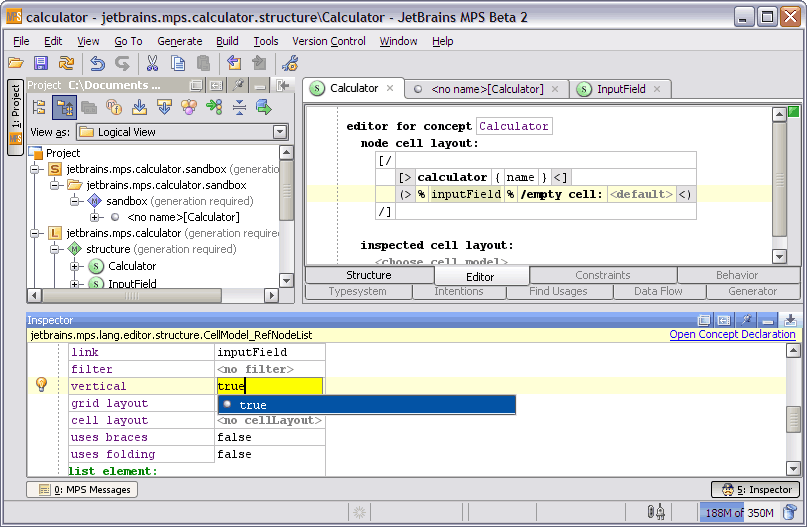
\includegraphics[scale=0.4]{img/mps.png}
\end{center}

\subsection{Среда Textual Modeling Framework(TMF) Xtext}
Аналог MPS для IDE Eclipse.
Набор инструментов для создания внешних DSL и редактора к ним на основе Eclipse.
Основано на технологиях Eclipse Modeling Framework(EMF), Graphical Modeling
Framework(GMF), Model To Text (M2T), Eclipse Modeling Framework Technology
(EMFT). На текущий момент (0.7.0RC1) проект находится на стадии разработки
(Eclipse incubation). Планируется интеграция в следующую версию Eclipse 3.5
Galileo.

В Xtext, в отличие от MPS, исходные файлы хранятся в обычном текстовом формате.

Грамматика одновременно с моделью задается с помощью компактного и
выразительного языка, в форме, похожей на сильно расширенную EBNF.

Xtext по грамматике языка создает:
\begin{itemize}
  \item инкрементальный парсер и лексер, основанный на ANTLR (в разработке
  собственный генератор парсеров packrat)
  \item мета модель, основанная на Ecore.
  \item сериализатор, используемый для преобразования мета модели обратно в
  текстовую форму, с сохранением исходного форматирования 
  \item интеграцию языка в Eclipse IDE:
  \begin{itemize}
    \item подсветка синтаксиса
    \item навигация (F3, и т.п.)
    \item автодополнение кода (ctrl-space)
    \item outline view
    \item шаблоны кода
  \end{itemize}
\end{itemize}

В качестве языка для генераторов кода, в Xtext используется Xpand
(статически-типизируемый шаблонный язык)

Пример описания языка в Xtext:
\begin{verbatim}
Model:
  (types+=Type)*;

Type:
  DataType | Entity;

DataType:
  "datatype" name=ID;

Entity:
  "entity" name=ID "{"
    (features+=Feature)* 
  "}";

Feature:
  type=[Type|ID] name=ID;   
\end{verbatim}

По мнению автора xtext хорошо подходит для создания малых языков предметной
области, но не для создания полноценных языков. 

\subsection{Среда Eclipse IDE Meta-Tooling Platform}
\label{imp}
Eclipse IMP - это набор инструментов для создания среды разработки для
произвольных языков.
Eclipse - это отличная среда для разработки на Java, но для
других языков программирования сделать подобную среду очень сложно. Цель
Eclipse IMP - упростить создание среды разработки на основе Eclipse для
произвольных языков.

В отличие от Xtext который ориентирован на небольшие языки предметной области
(DSL), IMP ориентирован на полноценные языки программирования. На основе IMP
были разработана среды для языков X10 и XJ, которые являются расширениями
языка Java.

Фактически IMP - это просто набор инструментов для создания сервисов к IDE для
разрабатываемого языка. В IMP интегрирован генератор парсеров LPG (ранее
известный как JikesPG), но возможно использование и других генераторов или
самописных парсеров.

Если компилятор генерирует Java файлы, IMP сможет даже их отлаживать благодаря
стандарту JSR-45~\cite{JSR45}. Для этого нужно в Java-файлы вставлять
комментарии вида ``//\#line'' для соответствия строк в исходном файле и сгенерированном по нему Java-файле.

IMP, LPG, X10, XJ - проекты компании IBM.

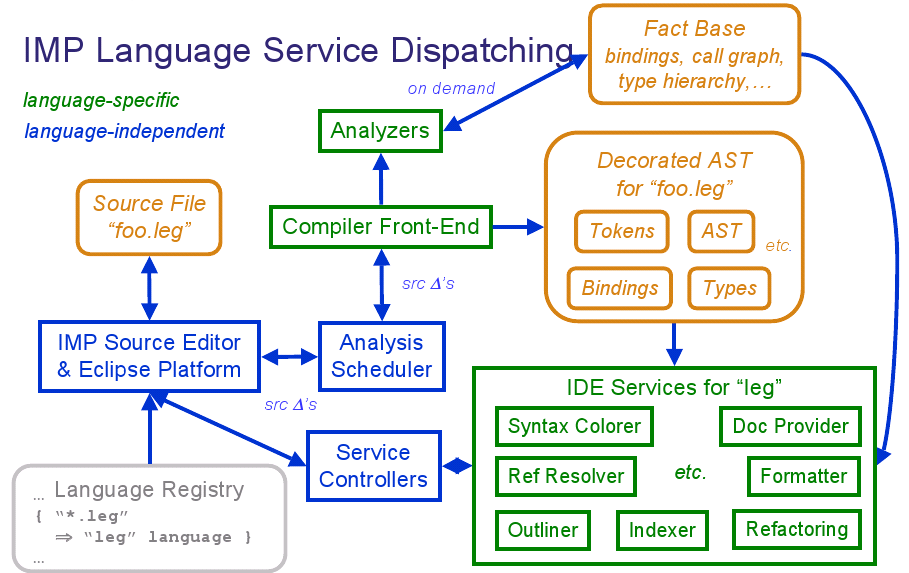
\includegraphics[scale=0.4]{img/imp.png}

\subsection{Генераторы парсеров}

\subsubsection*{yacc}
\begin{description}
  \item[распознаваемый класс языков]: LALR(1)
  \item[целевые ЯП]: yacc: C; bison: C, C++; и др.
  \item[особенности]: стандартизован в POSIX P1003.2. требует внешнего лексера: lex, flex.
\end{description}
yacc — стандартный генератор парсеров в Unix-системах. Название является
сокращением от «Yet Another Compiler Compiler» («всего лишь ещё один генератор
компиляторов»). Yacc генерирует парсер на основе аналитической грамматики,
описанной в нотации BNF. На выходе yacc выдаётся код парсера на языке
программирования Си.

Yacc был разработан Стивеном Джонсоном (Stephen C. Johnson) в компании AT\&T
для операционной системы Unix. Позже были написаны совместимые версии
программы, такие как Berkeley Yacc, GNU bison, MKS yacc и Abraxas yacc
(обновлённый вариант AT\&T-версии с открытым исходным кодом также вошёл в
проект OpenSolaris от Sun). Каждый вариант предлагал незначительные улучшения и
дополнительные возможности по сравнению с оригиналом, но концепция осталась той
же. Yacc также был переписан на других языках, включая Ratfor, EFL, ML, Ada,
Java, C\# и Limbo.

Парсер, генерируемый с помощью yacc, требует использования лексического
анализатора. В качестве него в большинстве случаев используется lex либо
flex. Стандарт IEEE POSIX P1003.2 определяет как функциональность так и
требования для lex и yacc.

Пример калькулятора на yacc
\begin{verbatim}
..
line   : exp ';' '\n'       {printf ("result is %d\n", $1);}
        ;
exp    : term               {$$ = $1;}
        | exp '+' term      {$$ = $1 + $3;}
        | exp '-' term      {$$ = $1 - $3;}
        ;
term   : factor             {$$ = $1;}
        | term '*' factor   {$$ = $1 * $3;}
        | term '/' factor   {$$ = $1 / $3;}
        ;
factor : number             {$$ = $1;}
        | '(' exp ')'       {$$ = $2;}
        ;
number : digit              {$$ = $1;}
        | number digit      {$$ = $1*10 + $2;}
..
\end{verbatim}

Как видно из примера, описание грамматики для yacc состоит из правил вывода и
некоторых действий, выполняемых при обнаружении данного вывода.
Yacc генерирует С-файл с парсером, который выполняет указанные действия.
Таким образом сгенерированный парсер НЕ строит дерева разбора. Его нужно строить
самостоятельно в действиях описания грамматики.

\subsubsection*{ANTLR}
\begin{description}
  \item[распознаваемый класс языков]: LL(*) (шире чем LALR(1))
  \item[целевые ЯП]: Java, C++, C\#, Python, Ruby
  \item[особенности]: наиболее мощный по возможностям. Требует специальную
  библиотеку для работы сгенерированного парсера (runtime dependency)
\end{description}
ANTLR — буквально Another Tool For Language Recognition (Ещё Одно Средство
Распознавания Языков) — генератор парсеров, позволяющий автоматически создавать
программу-парсер(как и лексический анализатор) на одном из целевых языков
программирования(С++, Java, C\#, Python, Ruby) по описанию LL(*)-грамматики на
языке, близком к EBNF. Позволяет конструировать компиляторы, интерпретаторы,
трансляторы с различных формальных языков. Предоставляет удобные средства для
восстановления после ошибок и сообщения о них. ANTLR — продолжение PCCTS(Purdue
Compiler Construction Tool Set), который был разработан в 1989 г.

Основоположником проекта и его главным вдохновителем является проф. Теренс Парр
(Terence Parr) из Университета Сан-Франциско. ANTLR — проект с открытым
исходным кодом, версия 3.1 распространяется по лицензии BSD. Проект в
настоящее время активно развивается.

Создатели ANTLR утверждают, что многие преимущества при определении действий
для правил являются следствием того, что ANTLR осуществляет LL разбор, то есть
использует разбор сверху вниз, в отличие от yacc, bison, которые
используют разбор снизу вверх. LL(*) разбор проще в понимании и
диагностике ошибок чем LR(1). К тому же класс языков распознаваемых LL(*)
разбором шире чем LR(1). Кроме того ANTLR выгодно отличается от других наличием
визуальной среды разработки ANTLRWorks, позволяющей удобно создавать и
отлаживать грамматики: это многооконный редактор, поддерживающий подсветку
синтаксиса, автодополнение, визуальное отображение грамматик, строящееся в
реальном времени по мере ввода, отладчик, инструменты для рефакторинга и т. д.

ANTLR, также как и yacc, выполняет указанные действия для правил вывода.

простейшая программа на ANTLR
\begin{verbatim}
grammar T;
//нетерминальные символы:
msg : 'name' ID ';' 
	{
		System.out.println("Hello, "+$ID.text+"!");
	} ;
//терминальные символы:
ID: 'a'..'z' + ;	//произвольное ( но >=1) количество букв
// пропускаемые символы:
WS: (' ' |'\n' |'\r' )+ {$channel=HIDDEN;} ;  пробел, перенос строки, табуляция
\end{verbatim}

\subsubsection*{ANTLR: Tree Parser}
ANTLR, как и yacc, не строит дерево разбора автоматически. Но у него есть
инструмент Tree Parser для его построения.

Если в описании грамматики не указывать действий, то на выходе парсера получится
просто список токенов. TreeParser позволяет указать в описании грамматики
правила для построения дерева из этих токенов, а также оперировать этим деревом.
Например заменить набор токенов узлом дерева, которое содержит эти токены в
качестве детей.

Таким образом, дерево разбора в ANTLR это просто дерево из токенов. Оно не
типизировано (значение токена всегда текст), и не структурировано (нет
информации о структуре узлов дерева: количестве детей, их типе).

\subsubsection*{ANTLR: Наследование грамматик}
У ANTLR начиная с версии 3.1 есть уникальная (за исключением LPG) в своем роде
возможность наследования грамматик. Эта возможность позволяет расширять
грамматики, дописывая новые правила вывода и заменяя старые. В результате
получается производный от базового класс парсера. Причем для наследования не
обязателен даже исходный код базового парсера. Наследование работает на
бинарном уровне, добавляя и перекрывая методы в производном классе парсера.

\subsubsection*{JavaCC}
Ничем особым не выделяется, кроме 2х расширений: JJTree и JTB. Эти расширения
генерируют классы AST и их построение по описанию языка.


\subsubsection*{SableCC}
\begin{description}
  \item[распознаваемый класс языков]: LALR(1)
  \item[целевые ЯП]: Java. Через расширения: C++, C\#, Python, O'Caml
  \item[особенности]: генерирует строго типизированное AST и расширенный
 	шаблон ``посетитель''.
\end{description}

SableCC --- генератор парсеров и лексеров, отличающийся генерацией большой
объектно-ориентированной библиотеки, необходимой для распознавания и анализа
языка по простому описанию грамматики языка. В частности, генерируемая
библиотека включает строго типизированное синтаксическое дерево и классы для
его прохода (tree walkers). SableCC  также сохраняет четкую границу между
генерируемым кодом, и кодом, написаным программистом, что ведет к уменьшению
цикла разработки. Из недостатков можно отметить слабую диагностику ошибок,
присущую большинству LR парсеров.

SableCC был выбран автором для создания специального языка XWiki Query Language
(XWQL) \cite{xwql} для проекта XWiki.org. Проект XWiki совмещает wiki-систему и
своего рода среду разработки для пользователей. XWiki позволяет пользователям
писать скрипты на некоторых языках, используя модель данных XWiki, которая
включает в себя документы, классы, объекты. Для запросов в базу данных
используется Hibernate Query Language (HQL) --- SQL-подобный язык запросов, в
котором достаточно трудно выразима модель данных XWiki. В качестве примера
приведем запрос поиска всех статей (документов с объектом класса
XWiki.ArticleClass) определенной категории:
\begin{verbatim}
select doc from XWikiDocument as doc, BaseObject as obj, 
 DBStringListProperty as prop join prop.list list
where obj.name=doc.fullName and obj.className='XWiki.ArticleClass' 
 and obj.name<>'XWiki.ArticleClassTemplate'  and obj.id=prop.id.id
 and prop.id.name='category' and list='${category}'
order by doc.creationDate desc
\end{verbatim}
Этот же запрос на XWQL:
\begin{verbatim}
where doc.fullName <> 'XWiki.ArticleClassTemplate' 
and :category member of doc.object(XWiki.ArticleClass).category
\end{verbatim}
Удобный и простой язык запросов очень важен для XWiki, т.к. позволит простым
пользователям писать достаточно сложные запросы в своих скриптах, не имея
знаний о внутренней структуре системы хранения XWiki. Также язык важен для
планируемого перехода XWiki на другую систему хранения, т.к. позволит не менять
язык запросов, а просто написать транслятор в язык запросов новой системы
хранения. При проектировании языка это требование также было учтено.

XWQL является расширением языка JPQL \cite{jpql} с добавлением новых
синтаксических конструкций, выражающих модель данных XWiki. Язык транслируется
в HQL и выполняется обычным образом в системе хранения XWiki. SableCC хорошо
подошел для реализации XWQL. Он сгенерировал множество полезных инструментов,
которые в других генераторах парсеров пришлось бы писать вручную. Побочным
результатом стал грамматика JPQL, записанная в терминах SableCC, которую можно
повторно использовать в других проектах, поскольку она не содержит никаких
спецефичных для XWQL частей (благодоря принципу отделения генерируемого и
ручного кода), в отличие от многих других грамматик на ANTLR, JavaCC.

\subsubsection*{LALR parser generator (LPG)}
\begin{description}
  \item[распознаваемый класс языков]: LALR(1)
  \item[целевые ЯП]: Java, C, C++
  \item[особенности]: генерирует строго типизированное AST и расширенный
 	шаблон ``посетитель''; наследование грамматик; возможность поиска с возвратом
 	(backtracking)
\end{description}

LPG ранее известен как JikesPG. Используется в экспериментальном
высокопроизводительном компиляторе Jikes, расширениях языка Java - X10 и XJ.
Имеет интеграцию с IDE Eclipse в проекте Eclipse IMP, описаном в разделе~\ref{imp}.

\subsubsection*{Parser combinators}
В функциональном программировании популярным подходом к построению рекурсивных
синтаксических анализаторов является моделирование парсеров как функций и
определение функций высшего порядка (комбинаторов), которые снабжены
грамматическими конструкциями, такими как упорядочение, выбор и повторение.
Такие парсеры образуют примеры монад, алгебраических структур из математики,
которые доказали полезность при исследовании большого числа вычислительных
задач.

Приведем пример распознавания простого DSL используя parser combinators.
DSL выглядит примерно так:
\begin{verbatim} 
(buy 100 IBM shares at max USD 45,
 sell 50 CISCO shares at min USD 25,
 buy 100 Google shares at max USD 800
 ) for trading_account "SSS1234")
\end{verbatim}
Описание DSL на языке Scala с помощью parser combinators:
\begin{verbatim} 
import scala.util.parsing.combinator.syntactical._
object OrderDSL extends StandardTokenParsers {
  lexical.delimiters ++= List("(", ")", ",")
  lexical.reserved += ("buy", "sell", "shares", "at", 
    "max", "min", "for", "trading", "account")
  def instr = trans ~ account_spec
  def trans = "(" ~> repsep(trans_spec, ",") <~ ")"
  def trans_spec = buy_sell ~ buy_sell_instr
  def account_spec = "for" ~> "trading" ~> "account" ~> stringLit
  def buy_sell = ("buy" | "sell")
  def buy_sell_instr = security_spec ~ price_spec
  def security_spec = numericLit ~ ident ~ "shares"
  def price_spec = "at" ~ ("min" | "max") ~ numericLit
}
\end{verbatim}
Как видно, в классе просто описана грамматика DSL в форме, похожей на
стандартную EBNF. По этому классу далее строится парсер, распознающий данный
DSL.

\subsection{Адаптивные грамматики}
\label{adaptive}
Адаптивной грамматикой называют формальную грамматику, которая предоставляет
механизмы для добавления, удаления и изменения своих правил вывода.

Адаптивные грамматики делятся на императивные, декларативные и гибридные.
\begin{itemize}
  \item Императивные (или глобальные) адаптивные грамматики модифицируют правила
  вывода на основании некоего глобального состояния, зависящего от времени
  (номера шага, time) в распознавании.
  \item Декларативные (или локальные) адаптивные грамматики модифицируют правила
  вывода на основании текущей позиции в грамматике (пространстве, space).
  \item Гибридные (пространственно-временные) адаптивные грамматики объединяют
  возможности императивных и декларативных. Они могут менять правила вывода как
  в соответствии со временем, так и в соотвентствие с пространством.
\end{itemize}

Теория адаптивных грамматик начала активно развиваеться в 90-ых годах.
Адаптивные грамматики способны распознать контекстно-зависимые языки.
Существуют очень мало парсеров на основе адаптивных грамматик, например PAISLEI
\cite{paislei}. Также существует проблема алгоритмической сложности таких
парсеров, т.к. не все получаемые из адаптивных грамматик языки распознаются
линейно. Но существуют и линейно распознаваемые языки \cite{paislei}.

Адаптивные грамматики ценны для расширений языков программирования, т.к.
позволяют распознавать больший класс языков, учитывая контекстно-зависимую
информацию. С их помощью становятся возможными довольно сложные синтаксические
расширения.

\subsection{Проект модульного компилятора}
На основе изученной информации можно попробовать наилучшим образом
спроектировать модульный компилятор:

К ядру компилятора подключается набор модулей. Каждый модуль содержит
синтаксические и/или семантические расширения. Базовый язык также может быть
модулем.

Синтаксическое расширение описывается добавлением и/или модификацией правил
вывода к базовой грамматике. (Для этого можно воспользоваться преобразованиями
Add и Extract, описанными в статьях П.Егорова~\cite{Egor}) В итоге объединения
синтаксических расширений подключенных модулей строится общая грамматика.

Семантическое расширение может описываться шаблоном программирования
``посетитель'' (visitor), который после построения дерева разбора, проходит по
нему и выполняет нужные действия. Также для облегчения выражения семантики в
модулях удобно пользоваться АОП.

\subsection{Дизайн IDE для модульного компилятора}

На основе Eclipse IMP можно спроектировать дизайн среды для модульных
компиляторов.
Отдельный модуль компилятора будет представлен плагином к Eclipse, в котором
должна содержатся грамматика расширения языка. Другие модули могут ей
пользоваться при наследовании. У модуля также могут быть сервисы для разных
частей IDE (подсветка синтаксиса, outline, автодополнения и пр).

Пользователь выбирает модули компилятора. После этого система генерирует
итоговый компилятор и сервисы IDE к нему.

\section{Заключение}

В данной работе произведен обзор, классификация и структуризация исследований
по расширениям языков программирования.
TODO

\small
%\nocite{*}

\bibliographystyle{plain}
\bibliography{bibtex}

\end{document}
